\documentclass{article}

% if you need to pass options to natbib, use, e.g.:
%     \PassOptionsToPackage{numbers, compress}{natbib}
% before loading neurips_2024

% submissions should not be anonymous, so use the
% [preprint] option:
\usepackage[preprint]{neurips_2024}

\usepackage{graphicx}
\graphicspath{ {./images/}{../images/}{./overleaf_microplastic_project/images/} }

\usepackage{float}

% Use the booktabs package for improved table formatting
\usepackage{booktabs}

% to avoid loading the natbib package, add option nonatbib:
%    \usepackage[nonatbib,preprint]{neurips_2024}

\usepackage{amsmath}
\usepackage[utf8]{inputenc} % allow utf-8 input
\usepackage[T1]{fontenc}    % use 8-bit T1 fonts
\usepackage{hyperref}       % hyperlinks
\usepackage{url}            % simple URL typesetting
\usepackage{amsfonts}       % blackboard math symbols
\usepackage{nicefrac}       % compact symbols for 1/2, etc.
\usepackage{microtype}      % microtypography
\usepackage{xcolor}         % colors
\usepackage{multirow}
\usepackage{subcaption}
\usepackage{array}
\newcommand{\emailaddr}[1]{{\scriptsize\texttt{#1}}}

\title{Microplastic Identification Using AI-Driven Image Segmentation with Synthetic Ecological Context}

\author{
\begin{minipage}[t]{0.47\textwidth}
  \centering
  Alex Dils\\
  University of California, Berkeley\\
  \emailaddr{dils@berkeley.edu}\\[0.6em]
  Jack Spottiswood\\
  University of California, Berkeley\\
  \emailaddr{spottiswood@berkeley.edu}\\[0.6em]
  Dylan Karmin\\
  Massachusetts Institute of Technology\\
  \emailaddr{dkarmin@mit.edu}\\[0.6em]
  Win Cowger\\
  University of California, Riverside\\
  Moore Institute for Plastic Pollution Research\\
  \emailaddr{win@mooreplasticresearch.org}
\end{minipage}
\hfill
\begin{minipage}[t]{0.47\textwidth}
  \centering
  David Raymond\\
  Dartmouth College\\
  \emailaddr{david.w.raymond.29@dartmouth.edu}\\[0.6em]
  Samay Kodige\\
  University of California, Berkeley\\
  \emailaddr{samaykodige@berkeley.edu}\\[0.6em]
  Rikhil Kokal\\
  University of California, Berkeley\\
  \emailaddr{rikhilkokal@berkeley.edu}\\[0.6em]
  Christoph Sad\'ee\\
  Stanford University\\
  Division of Computational Medicine\\
  \emailaddr{sadee@stanford.edu}
\end{minipage}
}

\begin{document}

\maketitle

\begin{abstract}
  Conventional methods for microplastic identification in water samples are costly and require expert analysis. Here, we propose a deep learning segmentation framework to identify microplastics in microscopic images and evaluate whether synthetic ecological context improves generalization to cluttered environmental imagery. We labeled microplastic images from the Moore Institute for Plastic Pollution Research and use generative inpainting to supplement limited training data with diverse image/mask pairs. The benchmark compares real-only training against multiple synthetic data sources, including Stable Diffusion, GAN, SDXL inpainting, FLUX inpainting, Stable Diffusion 2 inpainting, fiber-focused inpainting, and texture-focused inpainting conditions. Downstream evaluation spans U-Net, U-Net++, DeepLabV3+, FPN, MONAI U-Net, SegFormer-B2, and YOLO11m-seg, with repeated random seeds and a held-out ecological microscopy test set. In the completed core benchmark, real-only training has the strongest condition-level mean Dice and IoU (0.613 and 0.491), outperforming the legacy synthetic sources. In the completed semantic inpainting comparison, SDXL inpainting gives the strongest inpainting mean Dice and IoU (0.443 and 0.347). The best completed inpainting run uses Stable Diffusion 2 inpainting with U-Net++ EfficientNet-B4 at seed 37, reaching held-out Dice 0.651 and IoU 0.531.
\end{abstract}

\section{Introduction}

Microplastic pollution poses a significant threat to the health of marine ecosystems and safe drinking water \cite{ziani2023}. Therefore, the ability to quickly, cheaply, and accurately analyze samples is an invaluable tool for scientists and public health officials worldwide. Large-scale microplastic analysis is hindered by a lack of cheap and accessible measuring equipment \cite{stock2020}. Microplastic analysis requires laboratory-intensive physical and chemical pretreatments to prepare samples. This workup often entails a combination of manual analysis and Fourier-transform infrared spectroscopy (FTIR) or Raman spectroscopy to measure polymer type and confidently identify microplastics \cite{primpke2020}. Manual particle identification using visual microscopy is error-prone because natural particles can resemble microplastics and microplastics can appear visually heterogeneous. Spectroscopic workflows are more specific, but their cost and throughput restrict access to well-funded research institutions and specialized monitoring programs.

Deep learning models have shown substantial potential in identifying and quantifying structures within images while remaining inexpensive at inference time compared with traditional laboratory instrumentation. In microplastic imaging specifically, prior studies have used object detection for rapid localization and counting, semantic segmentation for particle masks, and hybrid systems that localize particles before pixel-level extraction \cite{lorenzo2021,park2022mpnet,shi2022sem,hao2024}. These approaches are complementary. Detection is attractive when the practical goal is screening many images, counting candidate particles, or drawing bounding boxes for expert review. Segmentation is needed when the scientific endpoint depends on particle area, shape, boundary, morphology, or recovery, because a bounding box cannot distinguish a thin fiber from the surrounding ecological debris inside the same box.

The main barrier is data. Supervised segmentation requires diverse labeled images, but many annotated microscopic images of microplastics are laboratory-prepared samples: the microplastic is photographed after pretreatment, while sediment, fibers, bubbles, organic matter, and other ecological debris have been removed. Models trained only on laboratory-prepared samples can therefore encounter a domain shift when deployed on raw or minimally processed environmental imagery. Recent microplastic segmentation work has reached strong performance in controlled settings such as fluorescence microscopy, scanning electron micrographs, and curated morphology datasets \cite{park2022mpnet,shi2022sem,yao2025}. However, ecological brightfield images remain difficult because microplastics can be transparent, thin, fragmented, or visually similar to non-plastic debris. To address this limitation, we use generative image inpainting to insert labeled microplastic-like structures into ecological backgrounds, producing synthetic image/mask pairs that preserve segmentation labels while broadening environmental context.

The central question is whether synthetic ecological context improves segmentation in a way that is robust across generation methods and downstream segmentation architectures. A single generator-model pairing is not sufficient to answer that question. We therefore define a benchmark that crosses multiple synthetic training conditions with multiple segmentation backbones and repeated random seeds, while reserving an ecological held-out test set for final evaluation.

The contributions of this manuscript are:
\begin{itemize}
  \item a three-cohort microplastic segmentation dataset with an ecological held-out test set;
  \item a benchmark comparing real-only training against GAN, Stable Diffusion, SDXL, FLUX, and Stable Diffusion 2 synthetic ecological context conditions;
  \item a model matrix covering semantic segmentation and YOLO-style instance segmentation backbones;
  \item a locked ecological evaluation protocol for reporting segmentation metrics across data conditions and model families;
  \item a detection-track design for comparing no-synthetic, synthetic, full-synthetic, combined, and all-source training regimes.
\end{itemize}

\subsection{Prior Work and Segmentation Rationale}

Five ideas motivate this study. First, microplastic pollution is a large and persistent environmental problem. Plastic production, use, and disposal have created widespread contamination, and microplastics are now recognized as a threat to ecosystems, food safety, and drinking water \cite{geyer2017,ziani2023}. Detection remains difficult because particles vary in size, color, shape, and polymer type, while environmental samples contain visually similar debris and often require costly preparation, microscopy, FTIR, or Raman spectroscopy for confirmation \cite{hidalgo2012,stock2020,primpke2020}.

Second, AI-based analysis has shown promise for accelerating microplastic workflows. Zhang et al.\ review recent progress in AI-based microplastic imaging and describe how computer vision can support particle detection, identification, and quantification \cite{zhang2023}. Related studies have used deep learning to reconstruct low-quality FTIR and Raman spectra and to classify microbeads in wastewater images \cite{brandt2021,yurtsever2019}. These results suggest that learned models can reduce manual screening burden and help scale monitoring, especially when outputs are treated as candidate detections for expert or spectroscopic confirmation.

Third, the central limitation is the lack of diverse labeled training data. Supervised segmentation requires paired images and masks that cover the visual range of microplastic morphologies, background materials, imaging settings, and preparation protocols. Existing microplastic image resources and data-sharing infrastructure improve access and validation, but benchmark-ready datasets with ecological context and pixel-level labels remain limited relative to the variability of real samples \cite{sherrod2024,zhang2023}. This data constraint is especially important for segmentation because small foreground masks can be overwhelmed by debris-driven false positives.

Fourth, synthetic data has improved data-limited learning in other computer vision settings. Standard augmentation can increase invariance to rotations, crops, flips, and color changes, but it cannot create new background contexts \cite{shorten2019}. More expressive synthesis methods, including GAN-based image-to-image translation and latent diffusion or inpainting models, can generate new image appearances while preserving specified conditioning inputs \cite{isola2017,rombach2022,podell2023,lugmayr2022,suvorov2022,li2022mat}. For microplastic segmentation, this makes synthetic ecological context a plausible way to expand training diversity while retaining known binary masks.

Fifth, synthetic-data claims should be tested across multiple downstream models. Segmentation performance can depend on architecture, scale handling, decoder design, and training dynamics. U-Net, U-Net++, DeepLabV3+, Feature Pyramid Networks, SegFormer, and YOLO-style segmentation models represent different assumptions about feature extraction and mask prediction \cite{ronneberger2015,zhou2018,chen2018,lin2017,xie2021,yolo11}. Evaluating several model families is therefore necessary to distinguish a general benefit of synthetic ecological training data from an effect that only appears for one generator-model pairing.

\section{Methods}

\subsection{Dataset Design}

We collected and organized three distinct datasets for model development. The data design separates three roles that are often conflated in small computer-vision studies: a labeled source domain for supervised learning, an unlabeled ecological background domain for synthetic data generation, and a held-out ecological domain for final testing. This separation is important because the central question is not whether a model can fit laboratory-prepared images, but whether additional ecological context can improve performance on cluttered imagery that more closely resembles deployment conditions.

\begin{table}[H]
  \centering
  \caption{Datasets used for training, synthesis, and evaluation.}
  \label{tab:datasets}
  \begin{tabular}{p{0.14\textwidth}p{0.17\textwidth}rrp{0.32\textwidth}}
    \toprule
    \textbf{Cohort} & \textbf{Source type} & \textbf{Images} & \textbf{Masks} & \textbf{Role in study} \\
    \midrule
    Cohort 1 & Laboratory microplastic microscopy & 368 & 368 & Supervised real-image training source and microplastic mask source for inpainting. \\
    Cohort 2 & Ecological microscopy backgrounds & 733 & 0 & Background image source for synthetic ecological context generation. \\
    Cohort 3 & Ecological microplastic microscopy & 97 & 97 & Primary held-out test set for segmentation evaluation. \\
    \bottomrule
  \end{tabular}
\end{table}

Cohort 1 contains microscopic images prepared as laboratory microplastic samples from the Microplastic Image Explorer dataset provided by the Moore Institute for Plastic Pollution Research. These images are paired with manually produced binary masks and are used as the real supervised training source. Cohort 2 contains ecological background images depicting environmental scenarios without annotated microplastics. Cohort 3 contains held-out ecological images showing microplastics in different contexts. For Cohort 1 and Cohort 3, we manually segmented the microplastics in each image, creating binary masks where white regions represent microplastics and black regions represent non-microplastic areas. Microplastic morphologies include fibers, fragments, and films.

\begin{figure}[t]
    \centering
    
\includegraphics[width=0.85\textwidth]{fig_dataset_counts.pdf}
    \caption{Dataset scale for the benchmark. The study combines 368 labeled Cohort 1 laboratory images, 733 Cohort 2 ecological backgrounds, a 97-image Cohort 3 ecological test set, and multiple synthetic training folders.}
    \label{fig:dataset-counts}
\end{figure}

\begin{figure}[t]
    \centering
    
\includegraphics[width=0.9\textwidth]{fig_mask_coverage.pdf}
    \caption{Foreground mask coverage distributions. Microplastic masks occupy a small fraction of each image, making this a small-object segmentation problem where false positives from debris can dominate metrics.}
    \label{fig:mask-coverage}
\end{figure}

\subsection{Synthetic Data and Segmentation Workflow}

The experiment has two linked stages. First, synthetic ecological training data are generated by pairing Cohort 2 backgrounds with transformed Cohort 1 masks. Second, segmentation models are trained on real-only or real-plus-synthetic training sets and evaluated on the same held-out ecological test set.

\subsection{Synthetic Data Conditions}

Each training condition starts with the same labeled Cohort 1 training data. Synthetic conditions add one generated image/mask folder to that real training base. Table~\ref{tab:generation-conditions} lists the synthetic data conditions. All inpainting conditions use Cohort 2 ecological backgrounds and transformed Cohort 1 masks to generate image/mask pairs.

\begin{table}[H]
  \centering
  \caption{Training data conditions. Core conditions are paired with all seven segmentation models. Cohort 2 inpainting conditions are paired with the five semantic segmentation models.}
  \label{tab:generation-conditions}
  \begin{tabular}{lll}
    \toprule
    \textbf{Condition} & \textbf{Synthetic source} & \textbf{Models trained} \\
    \midrule
    Baseline Cohort 1 & None; real Cohort 1 only & Seven-model core set \\
    SD synthetic & Stable Diffusion-style generation & Seven-model core set \\
    GAN synthetic & GAN-based generation & Seven-model core set \\
    Gen1 synthetic & First-generation synthetic set & Seven-model core set \\
    Cohort 2 generated & Cohort 2 compositing generation & Seven-model core set \\
    Cohort 2 SDXL inpaint & SDXL inpainting & Five semantic models \\
    Cohort 2 FLUX inpaint & FLUX-style inpainting & Five semantic models \\
    Cohort 2 SD2 inpaint & Stable Diffusion 2 inpainting & Five semantic models \\
    Cohort 2 SD2 fiber inpaint & Stable Diffusion 2 fiber-focused inpainting & Five semantic models \\
    Cohort 2 SDXL texture inpaint & SDXL texture-focused inpainting & Five semantic models \\
    \bottomrule
  \end{tabular}
\end{table}

For the inpainting conditions, the generator receives an ecological background image and a corresponding binary mask. The image is passed through a latent representation, while the mask indicates the region to synthesize. A text prompt guides synthesis toward plausible microplastic structures. A representative prompt is:
\begin{quote}
\emph{a realistic microscope ecological water sample containing a visible microplastic fiber, natural debris, sharp focus}
\end{quote}
with a negative prompt discouraging cartoons, illustrations, fake texture, text, watermarks, and blur.

For image synthesis, masks from Cohort 1 are randomly rotated, scaled, translated, and dilated. These transformed binary masks define regions for inpainting within Cohort 2 images. The inpainting model uses the ecological background, binary mask, and text conditioning to synthesize microplastic-like content inside the masked region while preserving the surrounding ecological context. The binary mask is retained as the segmentation label for the generated image.

Each inpainting method produces 10,000 image/mask pairs. Generated examples are not used in the primary Cohort 3 test set. The pipeline records generated filename, background path, source mask path, seed, prompt, model identifier, and transformation metadata for each output.

We also include a separate fully novel text-to-image generation arm using Gemini native image generation, commonly referred to as Nano Banana \cite{google2026nanobanana}. Unlike the inpainting conditions, this arm does not condition on a source mask and therefore does not automatically produce segmentation labels. Its role is exploratory: it can generate new candidate microplastic microscopy images for qualitative review, later manual annotation, or future label-assisted workflows. It is excluded from quantitative segmentation and detection training until image-level labels, boxes, or masks are verified.

\begin{figure}[t]
    \centering
    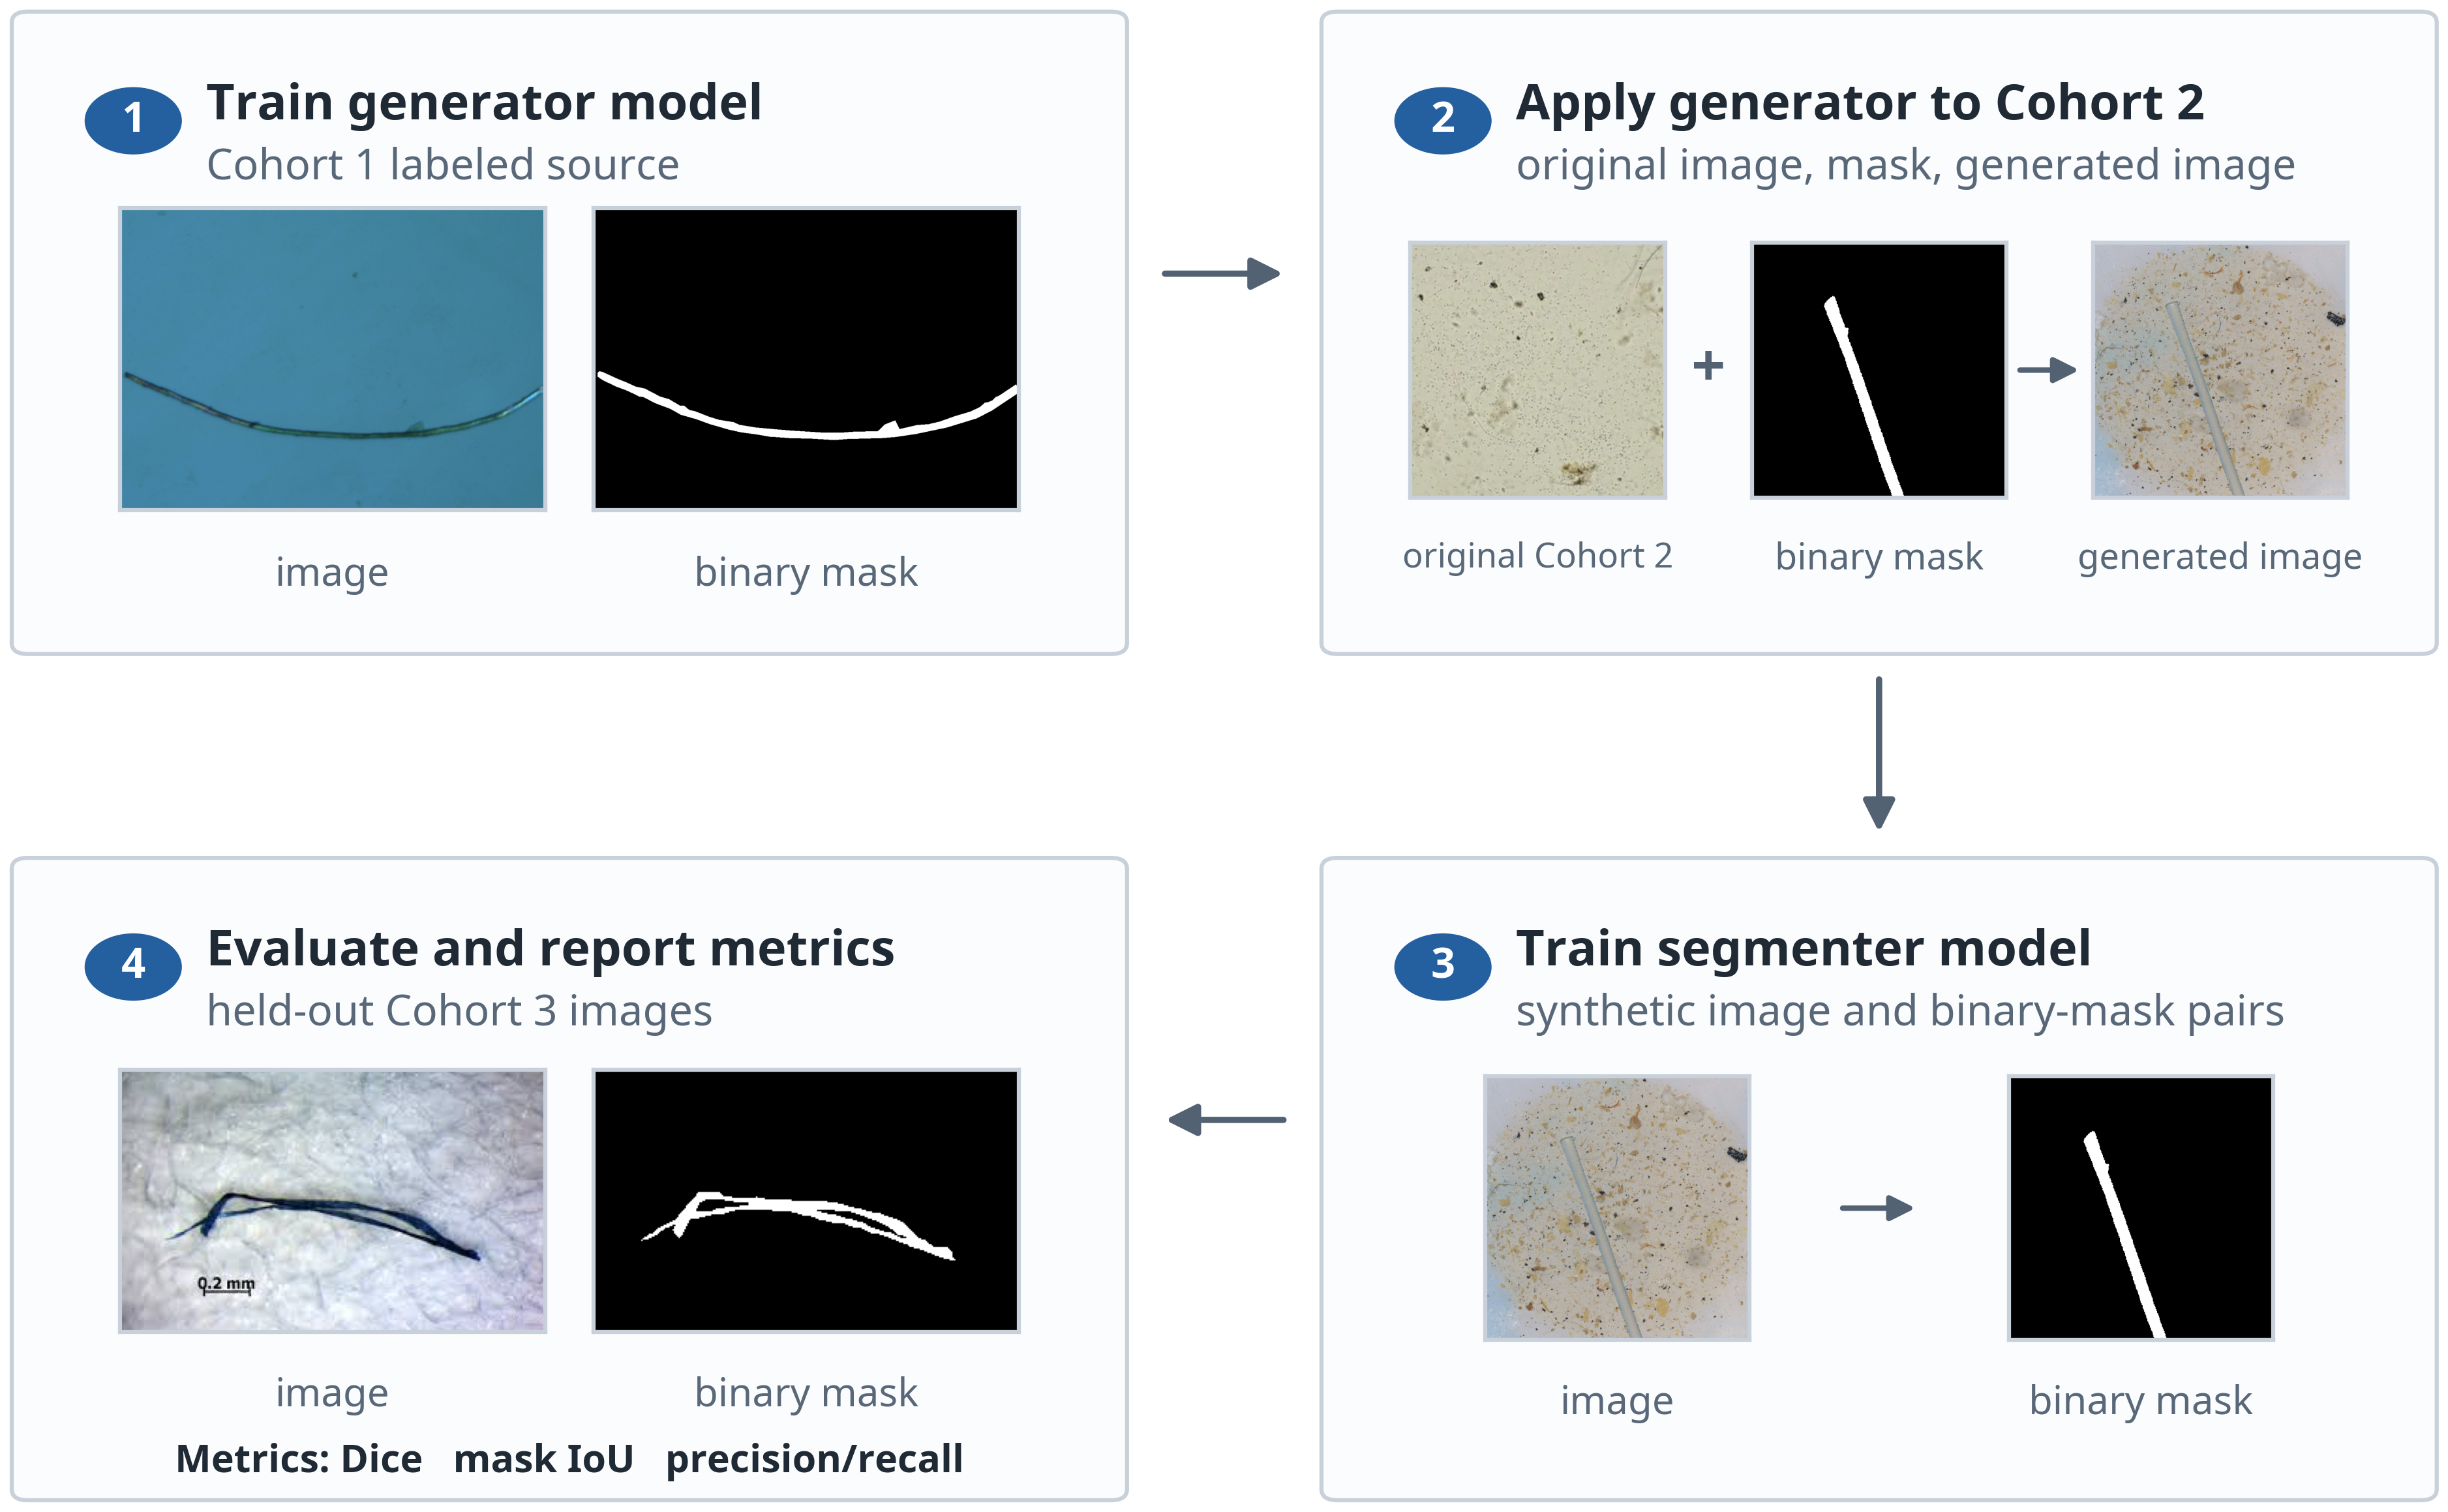
\includegraphics[width=\textwidth]{fig_workflow_complex.png}
    \caption{Workflow for synthetic ecological context generation and segmentation evaluation. Cohort 1 labeled data are used to train a generator model, the generator is applied to Cohort 2 ecological backgrounds to create synthetic training pairs, a segmenter is trained with the resulting data, and final metrics are computed on held-out Cohort 3 images.}
    \label{fig:pipeline}
\end{figure}

\subsection{Segmentation Models}

Table~\ref{tab:segmentation-models} lists all segmentation models included in the experiments. The seven-model core set contains five semantic segmentation models, one transformer segmentation model, and one YOLO-style instance segmentation model. The Cohort 2 inpainting comparison uses the five semantic segmentation models.

\begin{table}[H]
  \centering
  \caption{Segmentation models included in the benchmark.}
  \label{tab:segmentation-models}
  \begin{tabular}{lll}
    \toprule
    \textbf{Model} & \textbf{Architecture family} & \textbf{Condition set} \\
    \midrule
    smp\_unet\_resnet34 & U-Net, ResNet34 encoder & Core + Cohort 2 inpainting \\
    smp\_unetpp\_effb4 & U-Net++, EfficientNet-B4 encoder & Core + Cohort 2 inpainting \\
    smp\_deeplabv3plus\_resnet50 & DeepLabV3+, ResNet50 encoder & Core + Cohort 2 inpainting \\
    smp\_fpn\_effb3 & FPN, EfficientNet-B3 encoder & Core + Cohort 2 inpainting \\
    monai\_unet & MONAI U-Net & Core + Cohort 2 inpainting \\
    segformer\_b2 & SegFormer-B2 transformer & Core \\
    yolo11m\_seg & YOLO11m instance segmentation & Core \\
    \bottomrule
  \end{tabular}
\end{table}

Semantic models are trained as binary segmentation models using Dice+BCE loss. YOLO-style instance segmentation is trained after converting binary masks into polygon labels and is evaluated by merging predicted instances into a binary foreground mask. This allows semantic and instance-style models to be compared using the same downstream mask metrics.

\subsection{Segmentation and Detection Tracks}

We separate segmentation and detection because they answer different scientific and operational questions. The segmentation track is the primary analysis in this manuscript. It evaluates pixel-level masks with Dice, IoU, precision, recall, boundary F1, and foreground area error. These metrics are appropriate for estimating particle area, morphology, and boundary quality, which are central to microplastic burden estimation and source interpretation. Prior microplastic studies using MP-Net, U-Net variants, and newer multi-class segmentation models similarly motivate segmentation as a way to recover count, size, shape, and mask-based morphology rather than only image-level labels \cite{park2022mpnet,shi2022sem,yao2025}.

The detection track is included as a complementary screening benchmark. Detection models return bounding boxes and are useful for fast localization, counting, triage, and low-cost review workflows. This is why YOLO-style models appear in recent microplastic work, including studies that use object detection for rapid candidate localization before segmentation or confirmation \cite{lorenzo2021,hao2024,zahir2025}. For this project, the detection track uses boxes derived from the same binary masks so that detection and segmentation data splits remain comparable.

\begin{table}[H]
  \centering
  \caption{Detection-track training regimes. Box labels are derived from available binary masks. Fully novel text-to-image samples are excluded from quantitative detection training until manually annotated or otherwise label-verified.}
  \label{tab:detection-track}
  \begin{tabular}{lp{0.68\textwidth}}
    \toprule
    \textbf{Detection regime} & \textbf{Training data definition} \\
    \midrule
    No synthetic & Real labeled Cohort 1 images only. \\
    Synthetic & Real labeled images plus one selected mask-labeled synthetic source. \\
    Full synthetic & One selected mask-labeled synthetic source only, with no real images. \\
    Both & Real labeled images plus all available Cohort 2 inpainting synthetic sources. \\
    All together & Real labeled images plus every available mask-labeled synthetic source, including legacy and inpainting folders. \\
    \bottomrule
  \end{tabular}
\end{table}

The planned Nano Banana experiment is deliberately handled outside Table~\ref{tab:detection-track}. Because these generated images are fully novel and unlabeled, they are useful for testing visual plausibility and for estimating whether modern image-generation APIs can expand the space of microplastic morphologies. They are not used as ground truth for segmentation or detection metrics without a subsequent annotation step.

\subsection{Training Protocol}

All models use deterministic seeds 13, 37, and 101. Images are resized to 512$\times$512 during training. Training uses random horizontal and vertical flips, random translation, cropping, shear, and color jitter. Cohort 1 uses a fixed train/validation split, and synthetic folders are split deterministically into training and validation subsets. The Cohort 3 test set is never used for training, validation, threshold selection, prompt selection, or model selection.

\subsection{Generation and Training Settings}

Table~\ref{tab:appendix-generation-settings} lists the exact image generation settings used for the inpainting conditions. All generated images are resized to 512$\times$512, use transformed Cohort 1 masks as foreground labels, and use Cohort 2 images as ecological backgrounds. The mask transform samples rotation, scale, translation, and dilation before inpainting.

\begin{table}[H]
  \centering
  \scriptsize
  \setlength{\tabcolsep}{3pt}
  \caption{Generation model settings and prompts.}
  \label{tab:appendix-generation-settings}
  \begin{tabular}{@{}p{0.13\textwidth}p{0.16\textwidth}p{0.28\textwidth}p{0.18\textwidth}cc@{}}
    \toprule
    \textbf{Condition} & \textbf{Model ID} & \textbf{Prompt} & \textbf{Negative prompt} & \textbf{Guidance} & \textbf{Steps} \\
    \midrule
    Cohort 2 SDXL inpaint &
    diffusers/stable-diffusion-xl-\newline 1.0-inpainting-0.1 &
    a realistic microscope ecological water sample containing a visible microplastic fiber, natural debris, sharp focus &
    cartoon, illustration, fake texture, text, watermark, blurry &
    7.0 & 30 \\
    Cohort 2 FLUX inpaint &
    black-forest-labs/\newline FLUX.1-Fill-dev &
    a realistic microscope ecological water sample containing a microplastic particle, natural debris, sharp focus &
    cartoon, illustration, fake texture, text, watermark, blurry &
    3.5 & 28 \\
    Cohort 2 SD2 inpaint &
    stabilityai/stable-diffusion-2-\newline inpainting &
    microscope image of water sample with a translucent microplastic fragment inserted naturally, sharp focus &
    cartoon, illustration, fake texture, text, watermark, blurry &
    7.5 & 35 \\
    Cohort 2 SD2 fiber inpaint &
    stabilityai/stable-diffusion-2-\newline inpainting &
    real microscope water sample with an embedded blue microplastic fiber, natural illumination, sharp focus &
    cartoon, drawing, text, watermark, low resolution, blurry &
    8.0 & 45 \\
    Cohort 2 SDXL texture inpaint &
    diffusers/stable-diffusion-xl-\newline 1.0-inpainting-0.1 &
    a photorealistic microscope image with a colored microplastic fragment blended into sediment and organic debris &
    cartoon, illustration, fake texture, text, watermark, blurry, oversaturated &
    5.5 & 40 \\
    Nano Banana text-to-image &
    gemini-3.1-\newline flash-image &
    realistic optical microscope image of an environmental water sample containing new microplastic particles &
    not applicable &
    API default & API default \\
    \bottomrule
  \end{tabular}
\end{table}

Table~\ref{tab:appendix-training-settings} lists the segmentation training settings shared across models.

\begin{table}[H]
  \centering
  \caption{Segmentation training settings.}
  \label{tab:appendix-training-settings}
  \begin{tabular}{ll}
    \toprule
    \textbf{Setting} & \textbf{Value} \\
    \midrule
    Random seeds & 13, 37, 101 \\
    Image size & 512$\times$512 \\
    Batch size & 8 \\
    Maximum epochs & 80 \\
    Learning rate & 0.0001 \\
    Weight decay & 0.00001 \\
    Early stopping patience & 15 epochs \\
    Semantic loss & Dice + binary cross entropy \\
    Segmentation threshold & 0.5 \\
    Mixed precision & Enabled when CUDA is present \\
    Synthetic training split & 80\% train, 20\% validation \\
    Augmentation & Horizontal flip, vertical flip, translation, crop, shear, color jitter \\
    Primary evaluation set & Cohort 3, 97 images \\
    \bottomrule
  \end{tabular}
\end{table}

\subsection{Experimental Design}

The benchmark is organized around two questions. First, does adding synthetic ecological context improve segmentation relative to real-only Cohort 1 training? Second, do any gains hold across segmentation architectures rather than appearing only for a single backbone?

The core benchmark contains five data conditions, seven segmentation models, and three seeds, for \(5 \times 7 \times 3 = 105\) training runs. The Cohort 2 inpainting comparison contains five inpainting conditions, five semantic segmentation models, and three seeds, for \(5 \times 5 \times 3 = 75\) semantic segmentation runs. Each run is evaluated on the same Cohort 3 test set.

\subsection{Primary Metrics}

The primary endpoint for the expanded benchmark is Cohort 3 Dice and mask IoU:
\begin{equation}
\mathrm{Dice} = \frac{2TP}{2TP + FP + FN},
\qquad
\mathrm{IoU} = \frac{TP}{TP + FP + FN}.
\end{equation}
Secondary metrics are precision, recall, boundary F1, foreground area error, inference time, and parameter count. Predictions are resized back to original Cohort 3 image dimensions before scoring. Confidence intervals are computed by bootstrap resampling over Cohort 3 images.

\section{Results}

\subsection{Core Benchmark Results}

The completed core benchmark contains 105 evaluated checkpoints: five training conditions, seven segmentation models, and three random seeds. This matrix compares real-only training with four legacy synthetic training sources. Contrary to the expectation that every synthetic source would improve ecological generalization, the real-only baseline has the strongest condition-level average, with mean Dice 0.613 and mean IoU 0.491. Legacy GAN is the strongest synthetic condition in the core matrix, with mean Dice 0.524 and mean IoU 0.413.

\begin{table}[H]
  \centering
  \caption{Core benchmark performance by training condition. Values are mean $\pm$ standard deviation over seven segmentation models and three seeds.}
  \label{tab:core-condition-results}
  \begin{tabular}{lrrr}
    \toprule
    \textbf{Training condition} & \textbf{Runs} & \textbf{Dice} & \textbf{IoU} \\
    \midrule
    Baseline real only & 21 & 0.613 $\pm$ 0.153 & 0.491 $\pm$ 0.134 \\
    Legacy GAN synthetic & 21 & 0.524 $\pm$ 0.154 & 0.413 $\pm$ 0.127 \\
    Legacy Stable Diffusion synthetic & 21 & 0.473 $\pm$ 0.180 & 0.372 $\pm$ 0.145 \\
    Legacy Cohort 2 generated & 21 & 0.398 $\pm$ 0.180 & 0.306 $\pm$ 0.145 \\
    Legacy gen1 synthetic & 21 & 0.381 $\pm$ 0.207 & 0.293 $\pm$ 0.164 \\
    \bottomrule
  \end{tabular}
\end{table}

\begin{table}[H]
  \centering
  \caption{Core benchmark performance by segmentation model. Values are mean $\pm$ standard deviation over five training conditions and three seeds.}
  \label{tab:core-model-results}
  \begin{tabular}{lrrr}
    \toprule
    \textbf{Segmentation model} & \textbf{Runs} & \textbf{Dice} & \textbf{IoU} \\
    \midrule
    U-Net++ EfficientNet-B4 & 15 & 0.621 $\pm$ 0.071 & 0.502 $\pm$ 0.063 \\
    SegFormer-B2 & 15 & 0.616 $\pm$ 0.100 & 0.487 $\pm$ 0.096 \\
    FPN EfficientNet-B3 & 15 & 0.614 $\pm$ 0.076 & 0.488 $\pm$ 0.069 \\
    MONAI U-Net & 15 & 0.510 $\pm$ 0.139 & 0.386 $\pm$ 0.110 \\
    DeepLabV3+ ResNet50 & 15 & 0.362 $\pm$ 0.203 & 0.278 $\pm$ 0.164 \\
    YOLO11m-seg & 15 & 0.338 $\pm$ 0.134 & 0.261 $\pm$ 0.103 \\
    U-Net ResNet34 & 15 & 0.285 $\pm$ 0.197 & 0.222 $\pm$ 0.162 \\
    \bottomrule
  \end{tabular}
\end{table}

The best core run is the real-only baseline with SegFormer-B2 at seed 37, reaching held-out Dice 0.748 and IoU 0.627. These results motivate the follow-up ablation launched from this study: pure real, real plus inpainting, real plus Stable Diffusion synthetic images, pure synthetic, and pure inpainting training regimes.

\subsection{Inpainting Segmentation Results}

The completed semantic inpainting benchmark contains 75 checkpoints from a 75-run matrix: five inpainting conditions, five semantic segmentation models, and three random seeds. All 75 completed checkpoints were evaluated on the locked ecological test set. The 75 corresponding training histories are also present, and no runs in this matrix remain active. Validation metrics are reported only for training-health context; held-out ecological metrics are the primary evidence for generalization.

\begin{table}[H]
  \centering
  \caption{Execution status for the semantic inpainting benchmark.}
  \label{tab:current-status}
  \begin{tabular}{lr}
    \toprule
    \textbf{Status item} & \textbf{Count} \\
    \midrule
    Planned semantic inpainting runs & 75 \\
    Held-out evaluated completed checkpoints & 75 \\
    Training histories present & 75 \\
    Active training runs & 0 \\
    Not yet started runs & 0 \\
    \bottomrule
  \end{tabular}
\end{table}

Table~\ref{tab:c2-condition-results} summarizes held-out ecological performance by inpainting condition. SDXL inpainting has the strongest condition-level mean performance, with Dice 0.443 $\pm$ 0.126 and IoU 0.347 $\pm$ 0.103. Stable Diffusion 2 inpainting is second by mean Dice and IoU, followed by the SDXL texture-focused, Stable Diffusion 2 fiber-focused, and FLUX inpainting conditions.

\begin{table}[H]
  \centering
  \caption{Held-out ecological performance by Cohort 2 inpainting condition. Values are mean $\pm$ standard deviation over completed evaluated checkpoints.}
  \label{tab:c2-condition-results}
  \begin{tabular}{lrrrr}
    \toprule
    \textbf{Condition} & \textbf{Runs} & \textbf{Dice} & \textbf{IoU} & \textbf{Boundary F1} \\
    \midrule
    Cohort 2 SDXL inpaint & 15 & 0.443 $\pm$ 0.126 & 0.347 $\pm$ 0.103 & 0.500 \\
    Cohort 2 SD2 inpaint & 15 & 0.421 $\pm$ 0.183 & 0.328 $\pm$ 0.147 & 0.479 \\
    Cohort 2 SDXL texture inpaint & 15 & 0.406 $\pm$ 0.153 & 0.315 $\pm$ 0.121 & 0.461 \\
    Cohort 2 SD2 fiber inpaint & 15 & 0.398 $\pm$ 0.169 & 0.308 $\pm$ 0.136 & 0.453 \\
    Cohort 2 FLUX inpaint & 15 & 0.387 $\pm$ 0.148 & 0.300 $\pm$ 0.118 & 0.439 \\
    \bottomrule
  \end{tabular}
\end{table}

Model choice has a larger effect than the current differences among inpainting conditions. Table~\ref{tab:c2-model-results} shows that U-Net++ EfficientNet-B4 is the strongest model family, with mean Dice 0.569 $\pm$ 0.056 and IoU 0.459 $\pm$ 0.050. This pattern suggests that decoder capacity, multiscale features, and architecture remain central for small foreground segmentation under ecological clutter.

\begin{table}[H]
  \centering
  \caption{Held-out ecological performance by segmentation model. Values are mean $\pm$ standard deviation over completed evaluated checkpoints.}
  \label{tab:c2-model-results}
  \begin{tabular}{lrrrr}
    \toprule
    \textbf{Model} & \textbf{Runs} & \textbf{Dice} & \textbf{IoU} & \textbf{Boundary F1} \\
    \midrule
    U-Net++ EfficientNet-B4 & 15 & 0.569 $\pm$ 0.056 & 0.459 $\pm$ 0.050 & 0.635 \\
    MONAI U-Net & 15 & 0.506 $\pm$ 0.043 & 0.380 $\pm$ 0.037 & 0.579 \\
    FPN EfficientNet-B3 & 15 & 0.488 $\pm$ 0.045 & 0.383 $\pm$ 0.036 & 0.557 \\
    DeepLabV3+ ResNet50 & 15 & 0.328 $\pm$ 0.074 & 0.249 $\pm$ 0.060 & 0.382 \\
    U-Net ResNet34 & 15 & 0.162 $\pm$ 0.063 & 0.126 $\pm$ 0.049 & 0.179 \\
    \bottomrule
  \end{tabular}
\end{table}

The best completed single run is Cohort 2 SD2 inpaint with U-Net++ EfficientNet-B4 at seed 37, which achieves held-out Dice 0.651 with a 95\% bootstrap confidence interval of 0.595--0.703 and IoU 0.531 with a 95\% bootstrap confidence interval of 0.480--0.579. These top-run results show that synthetic ecological inpainting can support useful segmentation when paired with a strong segmentation architecture, but the spread across seeds and models cautions against drawing conclusions from any single generator-model pairing.

\begin{table}[H]
  \centering
  \caption{Training-validation summary by condition. These values monitor training health and checkpoint selection; they are not substitutes for held-out ecological metrics.}
  \label{tab:validation-condition-results}
  \begin{tabular}{lrrrr}
    \toprule
    \textbf{Condition} & \textbf{Runs} & \textbf{Best val Dice} & \textbf{Best val IoU} & \textbf{Last val Dice} \\
    \midrule
    Cohort 2 FLUX inpaint & 15 & 0.963 $\pm$ 0.013 & 0.933 $\pm$ 0.023 & 0.961 \\
    Cohort 2 SD2 inpaint & 15 & 0.963 $\pm$ 0.013 & 0.932 $\pm$ 0.023 & 0.962 \\
    Cohort 2 SDXL texture inpaint & 15 & 0.962 $\pm$ 0.013 & 0.932 $\pm$ 0.024 & 0.961 \\
    Cohort 2 SDXL inpaint & 15 & 0.962 $\pm$ 0.013 & 0.932 $\pm$ 0.024 & 0.959 \\
    Cohort 2 SD2 fiber inpaint & 15 & 0.962 $\pm$ 0.013 & 0.932 $\pm$ 0.024 & 0.959 \\
    \bottomrule
  \end{tabular}
\end{table}

The earlier single-condition smoke validation remains useful as an end-to-end check of the pipeline. This run trained a U-Net with a ResNet34 encoder using one seed on an SDXL-inpainted Cohort 2 synthetic training condition, then evaluated the resulting checkpoint on the 97-image Cohort 3 test set.

\begin{table}[H]
  \centering
  \caption{Preliminary single-condition Cohort 3 validation metrics. This run validates the end-to-end evaluation workflow; the full benchmark is required for condition-level conclusions.}
  \label{tab:preliminary-validation}
  \begin{tabular}{lcc}
    \toprule
    \textbf{Metric} & \textbf{Mean} & \textbf{95\% bootstrap CI} \\
    \midrule
    Dice & 0.067 & 0.041--0.096 \\
    Mask IoU & 0.041 & 0.024--0.061 \\
    Precision & 0.189 & -- \\
    Recall & 0.051 & -- \\
    Boundary F1 & 0.085 & -- \\
    Foreground area error & 0.015 & -- \\
    \bottomrule
  \end{tabular}
\end{table}

Because this smoke run uses one synthetic condition, one architecture, and one seed, we interpret it only as pipeline validation rather than final evidence for a synthetic-data benefit. The completed semantic inpainting benchmark provides stronger evidence because it aggregates multiple inpainting conditions, models, and seeds. The difference between high validation Dice values in Table~\ref{tab:validation-condition-results} and lower held-out Dice values in Tables~\ref{tab:c2-condition-results}--\ref{tab:c2-model-results} is scientifically important: it shows that within-condition validation performance can overstate ecological generalization. The benchmark therefore reports held-out ecological metrics as the primary outcome.

\section{Discussion}

The current results support three observations. First, synthetic ecological context is not sufficient by itself; architecture matters substantially. U-Net++ EfficientNet-B4, MONAI U-Net, and FPN EfficientNet-B3 are much stronger than U-Net ResNet34 on the same held-out ecological images. This suggests that the task benefits from models that preserve fine detail while incorporating broader context, because microplastic masks are small and often visually confounded by fibers, sediment, bubbles, and organic debris.

Second, the completed inpainting matrix shows that generation method matters, but the differences among inpainting conditions are smaller than the differences among segmentation architectures. SDXL inpainting has the highest condition-level mean, followed by Stable Diffusion 2 inpainting and SDXL texture-focused inpainting. The condition ranking should therefore be interpreted as evidence about this benchmark and training protocol rather than as a universal ordering of image-generation methods.

Third, the gap between validation and held-out ecological performance is a central result rather than a nuisance. Most completed training runs reach validation Dice near 0.94--0.96, yet held-out Dice is much lower. This is consistent with a real ecological domain shift: validation images share the synthetic generation process and training distribution, while the held-out ecological images contain real foregrounds, background clutter, and acquisition variability. The benchmark is designed around that gap, because the practical value of the model depends on performance outside the synthetic validation distribution.

For deployment, these models should be treated as screening tools rather than chemical-identification tools. A high-quality mask can prioritize candidate particles, support counting and area estimation, and reduce manual review time. It does not establish polymer identity. Downstream expert inspection, FTIR, Raman spectroscopy, or another confirmatory method remains necessary when material classification is required.

The performance level should also be interpreted in the context of prior microplastic image-analysis results. MP-Net reported mean F1 0.736 and mean IoU 0.617 on fluorescence microscopy images of microplastics isolated from clams \cite{park2022mpnet}. Shi et al.\ used SEM images and U-Net/MultiResUNet-style segmentation for quantification and shape classification, benefiting from high-resolution particle structure and a more controlled imaging modality \cite{shi2022sem}. Hao et al.\ reported very high performance for adherent microplastics in optical micrographs using a two-level YOLOv5 and UNET3+++ workflow, including a reported segmentation F1 of 99.65\% in that controlled biological-image setting \cite{hao2024}. More recently, Yao et al.\ used the Moore Institute image resource for multi-class microplastic segmentation and emphasized that segmentation provides location, shape, and area information that classification cannot provide \cite{yao2025}. Our current best held-out Dice of 0.651 and IoU of 0.531 is lower than the strongest controlled-setting reports, but that is not surprising: this benchmark evaluates ecological brightfield generalization under clutter, uses synthetic ecological training data, and reserves the held-out ecological test set from generation, validation, threshold selection, and model selection.

This context clarifies why segmentation is the primary endpoint. Detection can answer whether a candidate particle is present and roughly where it is, which is valuable for throughput and human review. Segmentation answers how much foreground is present and what morphology it has. For environmental monitoring, area, length, fiber shape, fragment shape, and particle boundaries can affect estimates of exposure and source attribution. A detection-only model can be useful as the first stage of a practical pipeline, but a segmentation model is better aligned with quantitative microplastic burden and morphology measurements.

\subsection{Reproducibility and Availability}

The benchmark is organized around deterministic manifests, fixed seeds, recorded generation metadata, and a locked Cohort 3 evaluation set. Each training run writes its configuration, training history, best checkpoint, and Cohort 3 metric summary. Synthetic generation records the source background, transformed mask, prompt, model identifier, seed, and transformation metadata for each generated pair. This structure is designed to make each result traceable from final metric back to image source, mask source, and training condition.

The code and data used in this study are publicly accessible. The code for the deep learning segmentation models and inpainting pipeline is available in the \href{https://github.com/axel-slid/Microplastic-Segmentation-GAN/tree/main}{project repository}, and the datasets used for training and evaluation are provided through the \href{https://dataverse.harvard.edu/dataverse/Microplastic-Segmentation-GAN/}{Harvard Dataverse archive}.

\subsection{Limitations}

There are several limitations to consider. First, generated images, although visually plausible, may not capture the full variability and complexity of real-world ecological scenarios. Synthetic foregrounds may also encode generator-specific artifacts that improve benchmark performance without improving field reliability. Second, the dataset may not encompass all environmental contexts where microplastics occur, which may limit generalization to new sites, imaging devices, particle morphologies, or preparation protocols.

The reported metrics are image-segmentation metrics rather than polymer-confirmation metrics. A predicted mask identifies candidate microplastic regions in an image, but chemical confirmation still requires expert review or spectroscopy when material identity is required. The method is therefore best understood as a scalable image-screening workflow that can prioritize samples and particles for downstream confirmation.

The Nano Banana generation arm has an additional limitation: it is an image source rather than a labeled dataset. Its outputs may broaden visual diversity, but they can also hallucinate morphology, optics, or background structure that is not representative of physical microplastic samples. We therefore treat Nano Banana images as candidates for qualitative inspection or downstream annotation, not as direct evidence for model performance.

\section{Conclusion}

This paper defines a scalable benchmark for microplastic identification using deep-learning segmentation models and synthetic ecological context. The experimental design compares real-only training against GAN, Stable Diffusion, SDXL, FLUX, and Stable Diffusion 2 synthetic data conditions; evaluates seven segmentation models in the core comparison; and reserves an ecological Cohort 3 test set for final comparison. The completed inpainting results show that held-out ecological segmentation is feasible but difficult: the best completed checkpoint reaches Dice 0.651 and IoU 0.531, while condition-level averages remain lower and vary substantially by architecture. These results reinforce the need to evaluate synthetic-data claims across multiple models and seeds rather than relying on a single generator-model pairing.

The completed inpainting matrix provides a reproducible framework for comparing synthetic ecological training data, measuring cross-domain segmentation performance, and identifying architectures that are most promising for microplastic image-screening workflows. The next experimental step is to extend the ablation from inpainting variants to broader data-mixture regimes: pure real microplastic images, real plus inpainting, real plus synthetic generation, pure synthetic generation, and pure inpainting.

\paragraph{Acknowledgments.}

We thank the Moore Institute for Plastic Pollution Research for their dataset of microplastic images, which was instrumental to our model training. We also thank all members of the Coding Club at Sequoia High School for their support and advice during the project.

\medskip

{\small

\begin{thebibliography}{99}

\bibitem{ziani2023}
Ziani, K. et al. (2023) Microplastics: A real global threat for environment and food safety: A state of the art review. \textit{Nutrients} \textbf{15}(3):617. doi:10.3390/nu15030617.

\bibitem{stock2020}
Stock, F. et al. (2020) Pitfalls and limitations in microplastic analyses. \textit{Plastics in the Aquatic Environment - Part I. The Handbook of Environmental Chemistry}, vol. 111. Springer, Cham. doi:10.1007/698\_2020\_654.

\bibitem{primpke2020}
Primpke, S., Christiansen, S.H., Cowger, W., et al. (2020) Critical assessment of analytical methods for the harmonized and cost-efficient analysis of microplastics. \textit{Applied Spectroscopy} \textbf{74}(9):1012--1047. doi:10.1177/0003702820921465.

\bibitem{sabir2022}
Sabir, M.W. et al. (2022) Segmentation of liver tumor in CT scan using ResU-Net. \textit{Applied Sciences} \textbf{12}(17):8650. doi:10.3390/app12178650.

\bibitem{zhang2023}
Zhang, Y., Zhang, D., and Zhang, Z. (2023) A critical review on artificial intelligence-based microplastics imaging technology: Recent advances, hot-spots, and challenges. \textit{International Journal of Environmental Research and Public Health} \textbf{20}:1150. doi:10.3390/ijerph20021150.

\bibitem{geyer2017}
Geyer, R., Jambeck, J.R., and Law, K.L. (2017) Production, use, and fate of all plastics ever made. \textit{Science Advances} \textbf{3}:e1700782. doi:10.1126/sciadv.1700782.

\bibitem{hidalgo2012}
Hidalgo-Ruz, V., Gutow, L., Thompson, R., and Thiel, M. (2012) Microplastics in the marine environment: A review of the methods used for identification and quantification. \textit{Environmental Science \& Technology} \textbf{46}:3060--3075. doi:10.1021/es2031505.

\bibitem{sherrod2024}
Sherrod, H. et al. (2024) One4All: An open source portal to validate and share microplastics data and beyond. \textit{Journal of Open Source Software} \textbf{9}(99):6715. doi:10.21105/joss.06715.

\bibitem{brandt2021}
Brandt, J., Mattsson, K., and Hassell\"ov, M. (2021) Deep learning for reconstructing low-quality FTIR and Raman spectra: A case study in microplastic analyses. \textit{Analytical Chemistry} \textbf{93}:16360--16368. doi:10.1021/acs.analchem.1c03162.

\bibitem{yurtsever2019}
Yurtsever, M. and Yurtsever, U. (2019) Use of a convolutional neural network for the classification of microbeads in urban wastewater. \textit{Chemosphere} \textbf{216}:271--280. doi:10.1016/j.chemosphere.2018.10.084.

\bibitem{lorenzo2021}
Lorenzo-Navarro, J., Castrill\'on-Santana, M., S\'anchez-Nielsen, E., Zarco, B., Herrera, A., and Mart\'inez, I. (2021) Deep learning approach for automatic microplastics counting and classification. \textit{Science of The Total Environment} \textbf{765}:142728. doi:10.1016/j.scitotenv.2020.142728.

\bibitem{park2022mpnet}
Park, H., Park, S., de Guzman, M.K., Baek, J.Y., Cirkovic Velickovic, T., Van Messem, A., and De Neve, W. (2022) MP-Net: Deep learning-based segmentation for fluorescence microscopy images of microplastics isolated from clams. \textit{PLOS ONE} \textbf{17}(6):e0269449. doi:10.1371/journal.pone.0269449.

\bibitem{shi2022sem}
Shi, B., Patel, M., Yu, D., Yan, J., Li, Z., Petriw, D., Pruyn, T., Smyth, K., Passeport, E., Miller, R.J.D., and Howe, J.Y. (2022) Automatic quantification and classification of microplastics in scanning electron micrographs via deep learning. \textit{Science of The Total Environment} \textbf{825}:153903. doi:10.1016/j.scitotenv.2022.153903.

\bibitem{hao2024}
Hao, Y., Wang, P., Cui, M., Zeng, Z., Ma, S., Li, Y., Zou, T., Fang, X., and Lin, L. (2024) Automatic localization and segmentation of adherent microplastics in optical micrographs based on improved YOLOv5 and adaptive perceptual UNET 3+++. \textit{Biomedical Signal Processing and Control} \textbf{95}:106399. doi:10.1016/j.bspc.2024.106399.

\bibitem{zahir2025}
Zahir, B.A. et al. (2025) Deep-learning enabled rapid and low-cost detection of microplastics in consumer products following on-site extraction and image processing. \textit{RSC Advances}. doi:10.1039/D4RA07991D.

\bibitem{yao2025}
Yao, Y., Xu, W., and Fan, H. (2025) A deep learning approach for microplastic segmentation in microscopic images. \textit{Toxics} \textbf{13}(12):1018. doi:10.3390/toxics13121018.

\bibitem{shorten2019}
Shorten, C. and Khoshgoftaar, T.M. (2019) A survey on image data augmentation for deep learning. \textit{Journal of Big Data} \textbf{6}:60. doi:10.1186/s40537-019-0197-0.

\bibitem{isola2017}
Isola, P., Zhu, J.-Y., Zhou, T., and Efros, A.A. (2017) Image-to-image translation with conditional adversarial networks. \textit{CVPR}. doi:10.1109/CVPR.2017.632.

\bibitem{rombach2022}
Rombach, R., Blattmann, A., Lorenz, D., Esser, P., and Ommer, B. (2022) High-resolution image synthesis with latent diffusion models. \textit{CVPR}. doi:10.1109/CVPR52688.2022.01042.

\bibitem{podell2023}
Podell, D. et al. (2023) SDXL: Improving latent diffusion models for high-resolution image synthesis. \textit{arXiv:2307.01952}.

\bibitem{lugmayr2022}
Lugmayr, A. et al. (2022) RePaint: Inpainting using denoising diffusion probabilistic models. \textit{CVPR}. doi:10.1109/CVPR52688.2022.01117.

\bibitem{suvorov2022}
Suvorov, R. et al. (2022) Resolution-robust large mask inpainting with Fourier convolutions. \textit{WACV}. doi:10.1109/WACV51458.2022.00323.

\bibitem{li2022mat}
Li, W., Lin, Z., Zhou, K., Qi, L., Wang, Y., and Jia, J. (2022) MAT: Mask-aware transformer for large hole image inpainting. \textit{CVPR}. doi:10.1109/CVPR52688.2022.01049.

\bibitem{ronneberger2015}
Ronneberger, O., Fischer, P., and Brox, T. (2015) U-Net: Convolutional networks for biomedical image segmentation. \textit{MICCAI}, 234--241.

\bibitem{zhou2018}
Zhou, Z., Siddiquee, M.M.R., Tajbakhsh, N., and Liang, J. (2018) UNet++: A nested U-Net architecture for medical image segmentation. \textit{Deep Learning in Medical Image Analysis and Multimodal Learning for Clinical Decision Support}, 3--11.

\bibitem{chen2018}
Chen, L.-C., Zhu, Y., Papandreou, G., Schroff, F., and Adam, H. (2018) Encoder-decoder with atrous separable convolution for semantic image segmentation. \textit{ECCV}, 801--818.

\bibitem{lin2017}
Lin, T.-Y., Doll\'ar, P., Girshick, R., He, K., Hariharan, B., and Belongie, S. (2017) Feature pyramid networks for object detection. \textit{CVPR}, 2117--2125.

\bibitem{xie2021}
Xie, E., Wang, W., Yu, Z., Anandkumar, A., Alvarez, J.M., and Luo, P. (2021) SegFormer: Simple and efficient design for semantic segmentation with transformers. \textit{NeurIPS}.

\bibitem{yolo11}
Ultralytics. (2024) YOLO11 models documentation. \url{https://docs.ultralytics.com/models/yolo11/}.

\bibitem{google2026nanobanana}
Google AI for Developers. (2026) Nano Banana image generation. \url{https://ai.google.dev/gemini-api/docs/image-generation}.

\end{thebibliography}

}

\end{document}
